\section{Mass Spring System implementation on cloth}
The cloth model is represented by a grid of triangles with a given mass to each point and those triangles are connected by a series of springs.\par

There are three types of spring which are needed to get the characteristics of cloth: 
\begin{itemize}
	\item Structural springs: Handle extension and compression and are connected vertically and horizontally. 
	\item Shear springs: Handle shear stresses and are connected diagonally. 
	\item Bend springs: Handle bending stresses and are connected vertically and horizontally to every other point. 
\end{itemize}

In our cloth simulation, only structural springs and bend springs are used. We use structural springs for all triangles and bend springs for all the springs connected the neighboring triangles. As the two neighboring triangles can always maintain rectangular shapes, there is no need to use the Shear springs on it. See figure \ref{fig:springs} for an example.\par
\begin{figure}[h]
	\centering
	\begin{subfigure}{0.4\textwidth}
		\centering
		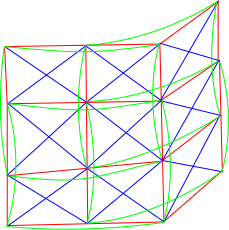
\includegraphics[width=0.6\textwidth]{springs_rectangular}
		\subcaption{Springs applied to a rectangular grid.}
		\label{fig:springs_rect}
	\end{subfigure}
	\quad
	\begin{subfigure}{0.4\textwidth}
		\centering
		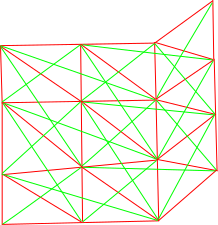
\includegraphics[width=0.6\textwidth]{springs_triangular}
		\subcaption{Springs applied to a triangular grid.}
		\label{fig:springs_triang}
	\end{subfigure}
	\caption{Example of a springs set up for a rectangular and a triangular grid. The structural springs are drawn in red color, bend springs are green colored. The blue shear springs are only applied to a rectangular grid.}
	\label{fig:springs}
\end{figure}

When the simulation is initiated, the rest length of each spring is set to the original length of the springs. The value of the masses and the stiffness of the springs are also set.\par

Once the masses and springs are all set up, and an environmental force, for example gravity, is applied to the points in the model over a specified time step, it produces a resulting acceleration for each point. This acceleration gives rise to a velocity which causes the point to update its position. The new position of each point in turn causes a change in length to each connected spring. The combination of the point and spring forces is integrated with respect to time to provide a new acceleration for each point. Calculating forces and updating positions iteratively provides the motion of the cloth object.

\subsection{Symplectic Euler method for mass-spring simulation}
To simulate the mass-spring network, a Symplectic Euler solver is implemented. Its benefit is a low computation effort in comparison to the other methods used during the pro-seminar. Unfortunately, the drawback is a less accurate result for each simulation step, which leads to integrated numeric errors. In our project accuracy is not important and so, they may be ignored as long the simulation stays stable.

\subsubsection{Algorithm}
For each time-step $h$ do the following steps:\par
For all mass-points compute position $\vec{x}$ at time $t+h$:
\begin{equation}
	\vec{x}(t+h) = \vec{x}(t) + h \cdot \vec{v}(t)
\end{equation}      
Compute forces $\vec{f}$ for all springs with end-points $\vec{x}_1$ and $\vec{x}_2$ at time $t$ considering the already updated values from $\vec{x}(t+h)$:
\begin{align}
	\vec{f}(t)          &= \vec{f}_{int}(t) + \vec{f}_{ext}(t) \text{ with} \\
	\vec{\Delta x}(t)   &= \vec{x}_1(t+h)-\vec{x}_2(t+h) \text{,}\\
	\vec{f}_{int}(t)    &= \frac{\vec{\Delta x}(t)}
	                       {||\vec{\Delta x}(t)||} \cdot k \cdot
	                       \left( l - ||\vec{\Delta x}(t)||\right) 
	                       \text{ and} \\
	\vec{f}_{ext}(t)    &= m \cdot \vec{g} + \vec{F}_P + \vec{f}_{interact}
\end{align}
The parameters $k$ and $l$ are the spring constants and rest lengths of the springs respectively. A ratio of $1 : 8$ for the spring constant $k$ between the bending- and structural springs gave reasonable results.
Interactive forces $\vec{f}_{interact}$ may be generated by any input devices like keyboard or mouse. Actually no interactions are implemented.
\par
Compute acceleration $\vec{a}$ for each point with mass $m$ at time $t$:
\begin{equation}
	\vec{a}(t) = \frac{1}{m} \cdot (\vec{f}(t) - \gamma \cdot \vec{v}(t))
\end{equation}
The damping parameter $\gamma$ is used to simulate friction and air pressure.
Finally, update the velocity $\vec{v}$ of each point at time $t+h$:
\begin{equation}
	\vec{v}(t+h) = \vec{v}(t) + h \cdot \vec{a}(t)
\end{equation}
